% Chapter Template

\chapter{Implementation} % Main chapter title

\label{Chapter5} % Change X to a consecutive number; for referencing this chapter elsewhere, use \ref{ChapterX}

In this section, I provide implementation-related details of my software prototype. The prototype is fully implemented and running on a set of nodes hosted by Google Cloud. I created four nodes in total, each with one virtual CPU and four gigabytes of RAM. On those nodes that host Cassandra, we reserve one gigabyte of RAM for Cassandra’s exclusive use and allow the remaining memory to be used by other components deployed on those nodes (such as Apache Spark). The nodes that host Cassandra are deployed using a native Kubernetes resource called \textit{stateful sets}. This data structure associates persistent volumes with particular system components such that data is preserved across restarts and crashes. They are designed to be used with distributed databases, like Cassandra, making it easy to add and remove nodes that host Cassandra at run-time. Thus, if we add a new node to our Cassandra cluster, Kubernetes ensures that a new persistent volume is created and attached to that node and then ensures that each time that component is activated the same persistent volume is made available to the database running on that node.

As mentioned above, we also designed our Kubernetes configuration to deploy an instance of an Apache Spark worker on each Cassandra node and then also specified one additional node to serve as the Apache Spark master node. A container with Zeppelin was also deployed configured to send queries to the Spark master node via Zeppelin’s cassandra-spark library.

I now present details on how each of the custom components discussed in Chapter~\ref{Chapter4} were implemented. In general, microservices were implemented first in python for ease of prototyping and then switched to a different implementation language if performance problems were detected. Furthermore, all microservices were placed in individual Docker containers which were then deployed via Kubernetes as dictated by the Infrastructure Manager. Further details on each component are now presented:

\begin{itemize}
	\item \textbf{Event Manager:} The event manager is implemented as a stateful django web application. It supports CRUD operations on events. Any change of state is pushed out as a message on a Kafka queue (and acted upon by the Infrastructure Controller). It stores its data in SQLite as a file on a Google Cloud persistent disk. This set-up ensures that it can find its state across restarts.

	\item \textbf{Infrastructure Controller:}  This controller is written in python and makes use of python libraries that allow it to interact with Kafka and Kubernetes. When it receives a message from the Event Manager, it issues commands to Kubernetes to declare the new state of the world. If an event is no longer active, its associated Tweet Normalizer is shut down. If a new event is specified, a new instance of the Tweet Normalizer is configured and deployed.

	\item \textbf{Twitter Tracker:} The Twitter Tracker was first implemented in Python but I discovered that python’s run-time engine was not fast enough to handle consistently high streaming volumes over long periods of time. As a result, I reimplemented this microservice in Go for better reliability and performance. As discussed above, this service submits keywords to Twitter’s Streaming API and then stores each tweet that it receives in a Kafka topic. The infrastructure controller is the one in charge of deploying and updating this service. A set of all the tracked keywords is passed as an environment variable on start by Kubernetes. To update the keywords, Kubernetes performs a rolling update by creating a new instance and destroying the old one, once the new one has correctly started the stream.

	\item \textbf{Twitter Normalizer:} The Twitter Normalizer is the one component in my infrastructure that can be instantiated multiple times and needs to monitor a different set of keywords in each instance. To facilitate this, I had the Infrastructure Controller direct Kubernetes to pass the keywords needed by each instance of the Twitter Normalizer via environment variables. Kubernetes could then deploy an instance of the Twitter Normalizer Docker container onto a node, configure its environment variables to match the keywords of the given event, and launch the microservice. The Twitter Normalizer was implemented in Python but specific C-based libraries were used to implement tasks that it executes over and over, e.g. loading and parsing JSON objects. This technique enabled the Twitter Normalizer to process the incoming stream of tweets with acceptable performance.
\end{itemize}

\section{Deploying the System}

Deploying my prototype is straightforward given the use of Google Cloud and Kubernetes. As mentioned above, I created a four-node cluster with each node allocated one virtual CPU and four gigabytes of RAM. Kafka and Cassandra/Spark are deployed first. In my prototype, I created two Kafka brokers that work together to manage the two primary topics needed by my design (the queue between the event manager and the infrastructure controller and the queue between the Twitter tracker and all instances of the Twitter normalizer) and instances of Cassandra/Spark on three of our four nodes. I then deployed the containers for my two front-end components: Zeppelin and the event manager. Finally, I deployed an instance of the infrastructure controller. All other components will be deployed by the infrastructure controller (including the Twitter tracker) when it receives a message from the event manager. This approach makes sense since there is no need to have the Twitter tracker and the Twitter normalizers running if there are no events to collect.

%\newpage

\section{Front-End Components}

Figure \ref{fig:eventmanager} shows the user interface of the event manager. Each event is shown in a separate box with information about the event’s keywords. There are controls for creating new events and a separate control for sending a message to the infrastructure controller with the most recent state of the world. Events can be edited/deleted by controls that appear when its box is selected. Figure \ref{fig:zeppelin} shows the user interface provided by Zeppelin. Queries can be submitted via a textbox and results can be displayed in tables or via bar graphs (as shown).

\begin{figure}
\centering
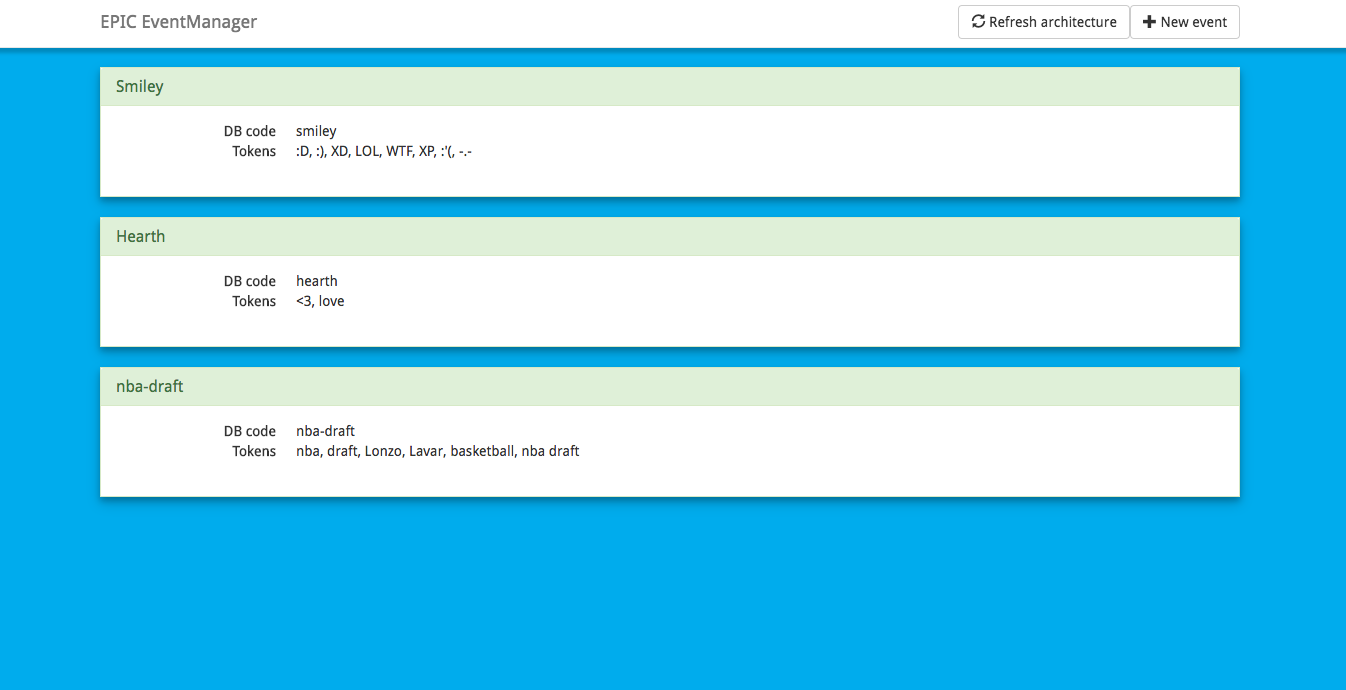
\includegraphics[width=\textwidth]{Figures/eventmanager}
\decoRule
\caption[Event Manager UI]{Event manager UI}
\label{fig:eventmanager}
\end{figure}

\begin{figure}
\centering
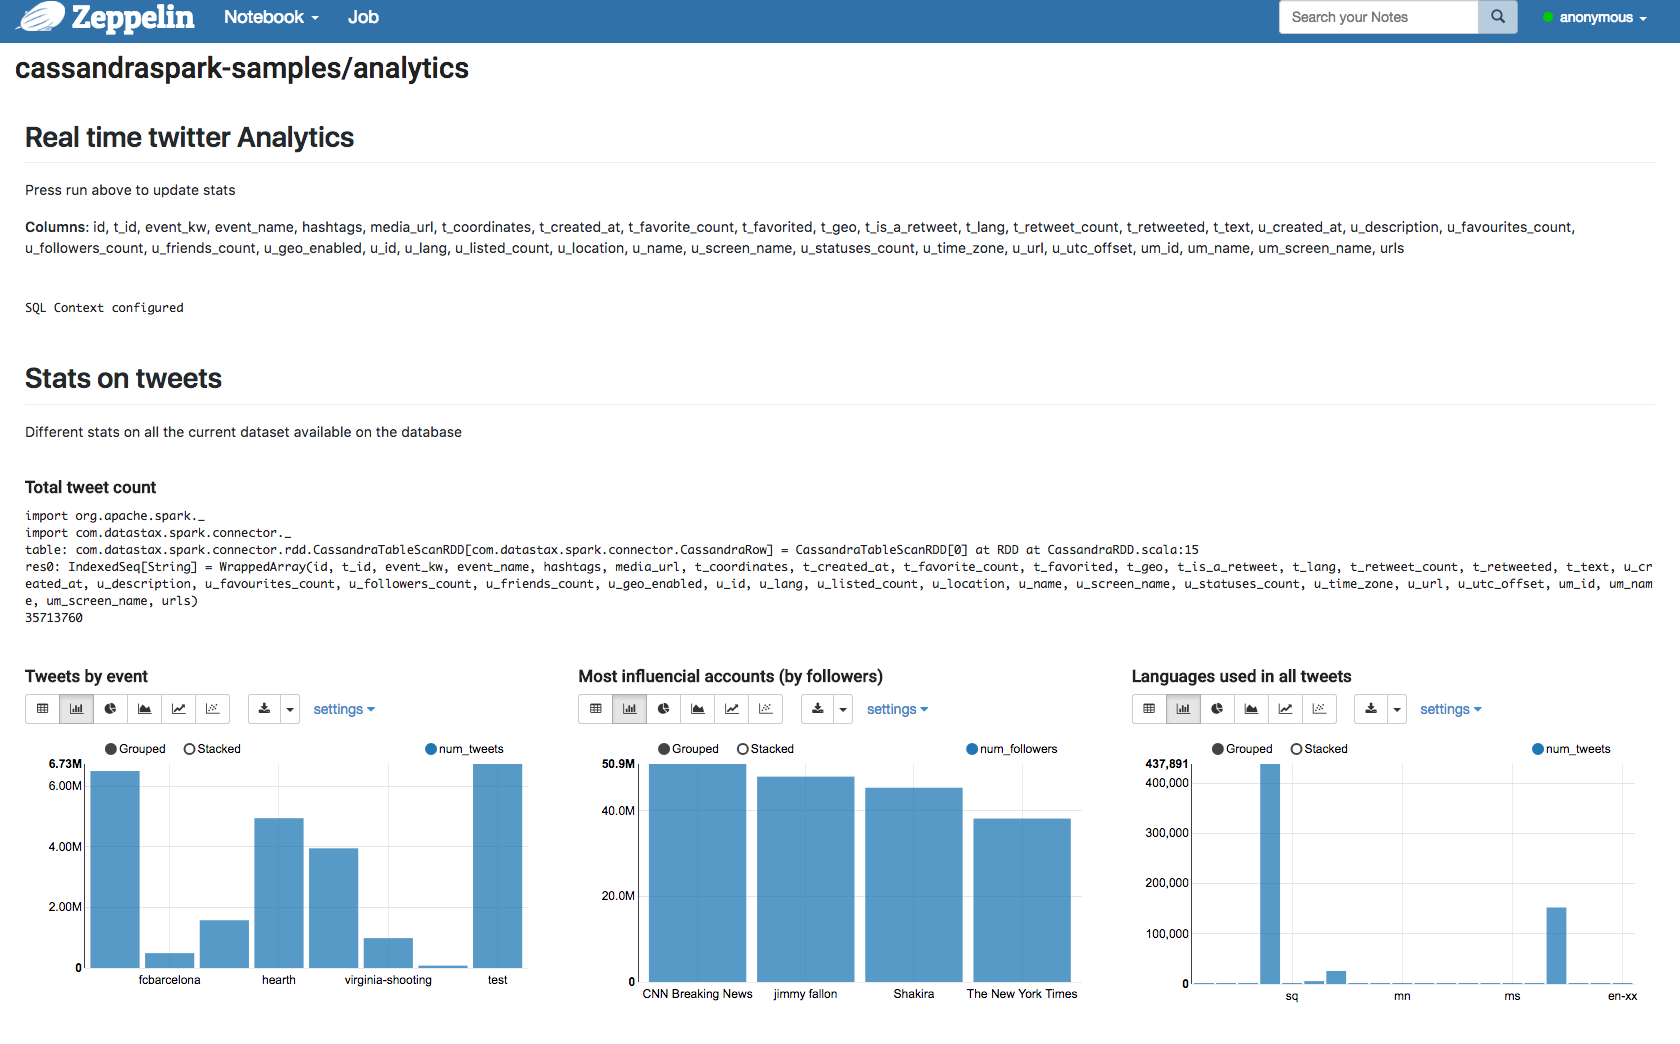
\includegraphics[width=\textwidth]{Figures/zeppelin}
\decoRule
\caption[Zeppelin visualization example]{Zeppelin server with some visualization from the dataset}
\label{fig:zeppelin}
\end{figure}
